% Generated by thesis/ch7/exp1/bench_figures.py -- do not edit by hand.
\begin{figure}[tbp]
  \centering
  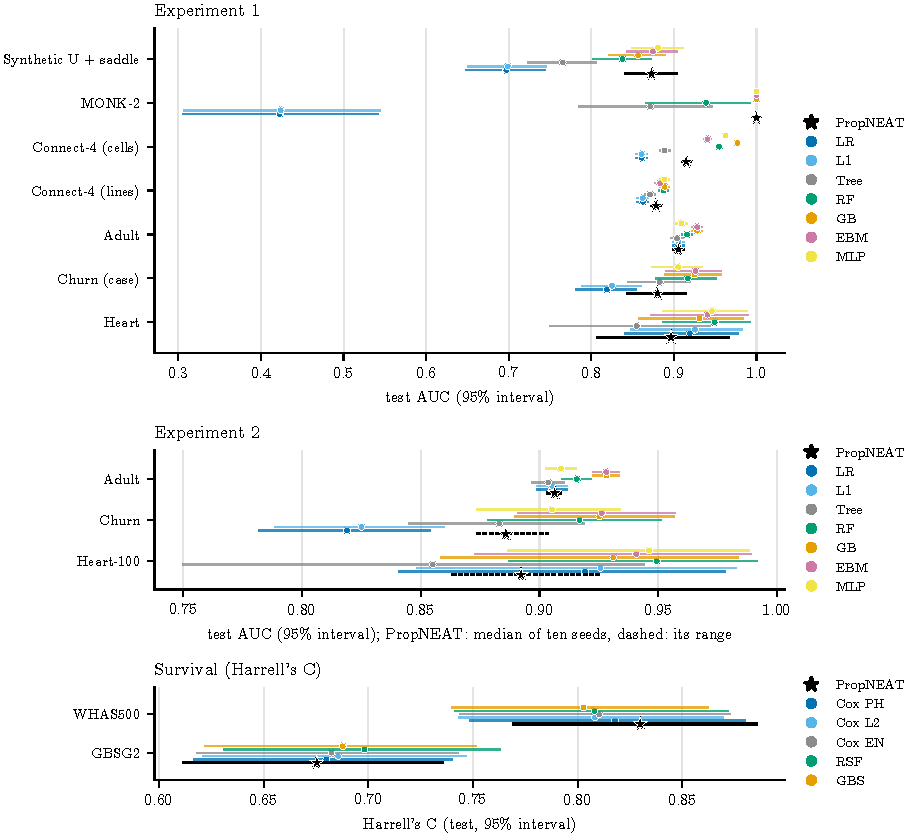
\includegraphics[width=\textwidth,height=0.8\textheight,keepaspectratio]{figures/ch7/bench-dots.pdf}
  \caption{Test AUC of PropNEAT and of each comparator, every dataset. Star: PropNEAT (Experiment 2: median of the ten seeds, dashed: their range); dots: comparators; lines: 95\% intervals; survival datasets: Harrell's C. LR: logistic regression ($L_2$); L1: $L_1$ logistic regression; RF: random forest; GB: gradient boosting; EBM: explainable boosting machine; MLP: multilayer perceptron; Cox L2 / Cox EN: Cox model with a ridge / elastic-net penalty; RSF: random survival forest; GBS: gradient-boosted survival model.}
  \label{fig:ch7-bench-dots}
\end{figure}
